\documentclass[12pt,letterpaper]{article}
\usepackage{fullpage}
\usepackage[top=2cm, bottom=4cm, left=2.5cm, right=2.5cm]{geometry}
\usepackage{amsmath,amsthm,amsfonts,amssymb,amscd}
\usepackage{lastpage}
\usepackage{enumerate}
\usepackage{fancyhdr}
\usepackage{mathrsfs}
\usepackage{xcolor}
\usepackage{graphicx}
\usepackage{listings}
\usepackage{hyperref}
\usepackage{float}

\hypersetup{%
  colorlinks=true,
  linkcolor=blue,
  linkbordercolor={0 0 1}
}
 
\renewcommand\lstlistingname{Algorithm}
\renewcommand\lstlistlistingname{Algorithms}
\def\lstlistingautorefname{Alg.}

\lstdefinestyle{Python}{
    language        = Python,
    frame           = lines, 
    basicstyle      = \footnotesize,
    keywordstyle    = \color{blue},
    stringstyle     = \color{green},
    commentstyle    = \color{red}\ttfamily
}

\setlength{\parindent}{0.0in}
\setlength{\parskip}{0.05in}
\begin{document}
Sunny Lee

\begin{enumerate}
    \item 
    \begin{enumerate}
        \item 
        Using Newton's method: \\
        In the interval $[0, \frac{1}{2}]$\\
        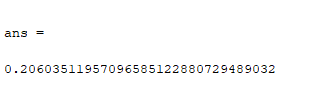
\includegraphics{number1aa.png}\\
        In the interval $[\frac{1}{2}, 1]$\\
        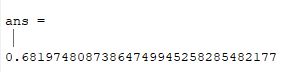
\includegraphics{number1ab.png}
        \item
        Using Secant method: \\
        In the interval $[0, \frac{1}{2}]$\\
        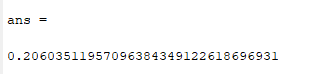
\includegraphics{number1ba.png}\\
        In the interval $[\frac{1}{2}, 1]$\\
        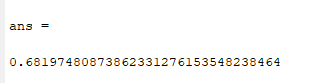
\includegraphics{number1bb.png}
        \item
        Using False Point method: \\
        In the interval $[0, \frac{1}{2}]$\\
        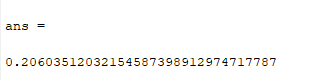
\includegraphics{number1cb.png}\\
        In the interval $[\frac{1}{2}, 1]$\\
        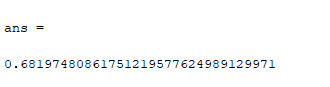
\includegraphics{number1ca.png}
    \end{enumerate}
    \item
    \begin{enumerate}
        \item 
        Using Newton's method: \\
        In the interval $[-\frac{1}{2}, \frac{1}{2}]$\\
        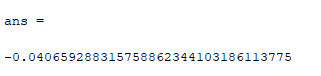
\includegraphics{number2aa.png}\\
        In the interval $[\frac{1}{2}, 1.5]$\\
        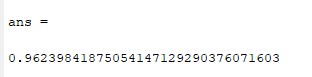
\includegraphics{number2ab.png}
        \item
        Using Secant method: \\
        In the interval $[-\frac{1}{2}, \frac{1}{2}]$\\
        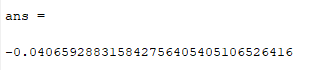
\includegraphics{number2ba.png}\\
        In the interval $[\frac{1}{2}, 1.5]$\\
        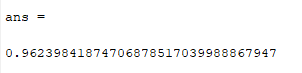
\includegraphics{number2bb.png}
        \item
        Using False Point method:\\
        In the interval $[-\frac{1}{2}, \frac{1}{2}]$\\
        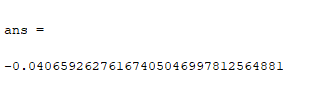
\includegraphics{number2ca.png}\\
        In the interval $[\frac{1}{2}, 1.5]$\\
        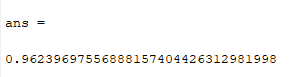
\includegraphics{number2cb.png}
    \end{enumerate}
    \item 
    The simpler formulation of the secant method only involves a fraction as the 
    $p_n$, so if the two terms in the numerator are very close, the machine 
    might round down to zero setting our $p_n$ to be zero. The formulation given 
    in the book, however, if the numerator terms round to zero, $p_n$ will be 
    equal to $p_{n-1}$ thus our $p_n$ will not jump to zero if the two numerator 
    terms are very close to one another.
\end{enumerate}

\end{document}